%!TEX root=../GaugeCNNTheory.tex


\section{مدل اسباب‌بازی: کانولوشن‌های موبیوس هموردای بازتابی}
\label{sec:mobius_conv}

برای ملموس‌تر کردن ملاحظات نظری در بخش‌های قبل، اکنون به یک کاربرد نمونه می‌پردازیم.
کانولوشن‌های $\GM$ روی نوار موبیوس، با اینکه اهمیت عملی فوری ندارند، یک مدل اسباب‌بازی مناسب هستند زیرا هندسه و نظریه نمایش درگیر در آن به طور خاص ساده هستند.
به دلیل عدم جهت‌گیری آن، چارچوب‌های مرجع را فقط می‌توان تا حد بازتاب‌ها به صورت (هموار) ارجح دانست.
همانطور که انتظار می‌رود، \CNN{}های مستقل از مختصات، که توابع الگوی هموردای بازتابی را اعمال می‌کنند، از یک پیاده‌سازی ساده و وابسته به مختصات بهتر عمل می‌کنند.
علاوه بر این، نشان داده می‌شود که آنها تحت عمل گروه ایزومتری نوار موبیوس هموردا هستند.

\etocsettocdepth{3}
\etocsettocstyle{}{} % from now on only local tocs
\localtableofcontents

بخش بعدی~\ref{sec:mobius_geometry} به بحث در مورد هندسه نوار موبیوس مسطح می‌پردازد.
به دلیل پیچش آن، گروه ساختار آن را نمی‌توان بیشتر از گروه بازتاب~$G=\Flip$ کاهش داد، به طوری که باید یک اطلس $\Flip$ از گیج‌ها را همانطور که در شکل~\ref{fig:mobius_conv_gauges} به تصویر کشیده شده است، در نظر گرفت.
گروه ایزومتری توسط دوران‌ها در امتداد نوار داده می‌شود و تبدیلات گیج $\Flip$-مقدار را القا می‌کند.
میدان‌های ویژگی $\RM$-مستقل از مختصات که برخی از آنها در بخش~\ref{sec:mobius_representations} معرفی شده‌اند، لزوماً باید مطابق با نمایشی از گروه بازتاب تبدیل شوند.
بخش~\ref{sec:mobius_cnn_ops_analytical} عملیات شبکه کانولوشنی مستقل از جهت‌گیری را مورد بحث قرار می‌دهد.
این بخش به طور خاص مفهوم کرنل‌های $G$-راهبر را روشن می‌کند اما بایاس‌ها و غیرخطی‌های هموردای بازتابی را نیز پوشش می‌دهد.
یک پیاده‌سازی عددی از خانواده مدل پیشنهادی در بخش~\ref{sec:mobius_experiment_main} مورد بحث و ارزیابی قرار می‌گیرد.
کد به صورت عمومی در آدرس \url{https://github.com/mauriceweiler/MobiusCNNs} در دسترس است.

\subsection{هندسه نوار موبیوس}
\label{sec:mobius_geometry}

خمینه $M$ مورد نظر، نوار موبیوس مسطح با مرز است که در شکل~\ref{fig:weight_sharing_ambiguity} (راست) نشان داده شده است.
می‌توان آن را به گونه‌ای تصور کرد که با گرفتن یک زیرمجموعه مستطیلی $[0,X] \times [0,Y]$ از $\R^2$ و چسباندن دو انتهای متقابل به روشی پیچ‌خورده ساخته شده است.
نوار موبیوس که اینگونه تعریف شده، متریک کانونی $\R^2$ را به ارث می‌برد که به آن یک ساختار ریمانی می‌بخشد.
این متریک به طور خاص یک اتصال لوی-چیویتا و در نتیجه نگاشت‌های نمایی و انتقال‌دهنده‌های موازی را مشخص می‌کند که در ادامه بیشتر مورد بحث قرار می‌گیرند.

\begin{figure}[H]
	\centering
	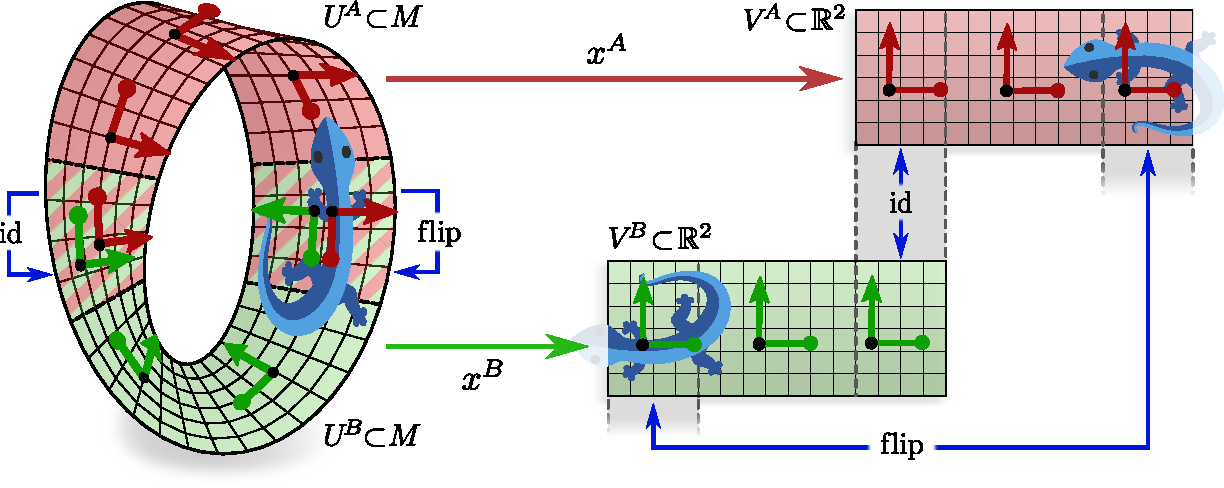
\includegraphics[width=\columnwidth]{figures/mobius_conv_gauges.pdf}
	\vspace*{.5ex}
	\caption{\small
		هندسه مسطح نوار موبیوس امکان وجود زیرمجموعه‌های محلی را فراهم می‌کند که می‌توانند به صورت ایزومتریک با زیرمجموعه‌های متناظر~$\R^2$ شناسایی شوند.
		ما یک اطلس ایزومتریک را ثابت می‌کنیم که شامل دو چارت $x^A$ و $x^B$ روی $U^A$ (قرمز) و $U^B$ (سبز) است که کل نوار را پوشش می‌دهند.
		گیج‌های $\psi_p^X := \hat{d}x_p^X: \TpM \to \R^d$ برای $p\in U^A$ به عنوان دیفرانسیل‌های چارت القا می‌شوند.
		به دلیل پیچش نوار موبیوس، توابع گذار $g_p^{BA}$ در یکی از نواحی همپوشانی بدیهی خواهند بود، در حالی که ناحیه دیگر لزوماً بین گیج‌ها از طریق بازتاب‌ها~$s$ گذار خواهد کرد.
		بنابراین، اطلس انتخاب‌شده از چارت‌ها یک اطلس $\Flip$ از گیج‌ها را القا می‌کند و یک ساختار $\Flip$ متناظر $\RM$ را ایجاب می‌کند که شامل دو چارچوب بازتاب‌شده در هر نقطه از~$M$ است.
		هر یک از چارت‌های $x^X$ یک میدان چارچوب هموار محلی را القا می‌کند که توسط پایه‌های مختصاتی
		$\bigl[\frac{\partial}{\partial x_i^X} \big|_p \bigr]_{i=1}^d$ داده می‌شود.
		بازتاب در توابع گذار در یک همپوشانی، به صورت بازتاب چارچوب‌ها نشان داده می‌شود.
		{
			\\ \color{gray} \scriptsize
			(مارمولک‌ها با مجوز \href{https://github.com/twitter/twemoji/blob/gh-pages/LICENSE-GRAPHICS}{\lr{\underline{Creative Commons Attribution 4.0 International}}} با تشکر از توییتر اقتباس شده‌اند.)
		}
	}
	\label{fig:mobius_conv_gauges}
\end{figure}

اولین سوالی که هنگام ساخت یک \CNN{} مستقل از مختصات باید به آن پاسخ داد این است که انتخاب چارچوب‌های مرجع تا چه حد مبهم است.
با توجه به متریک ریمانی روی نوار، می‌توانیم توجه خود را به چارچوب‌های متعامد محدود کنیم.
علاوه بر این، می‌توان یکی از دو جهت \emph{در امتداد} نوار را برای رفع ابهام (هموار) دوران چارچوب‌های مرجع با هم‌تراز کردن محورهای اول آنها با این جهت، مشخص کرد.
این کار ما را با ابهام دست‌سانی چارچوب مواجه می‌کند، که دو جهت‌گیری آن متناظر با دو جهت ممکن محور دوم چارچوب عمود بر نوار است.
نوار موبیوس به عنوان یک خمینه غیرقابل جهت‌گیری، یک انتخاب هموار (یا حتی پیوسته) سراسری از جهت‌گیری‌های چارچوب را نمی‌پذیرد.
برای به دست آوردن شهودی از این گزاره، تلاش برای ساخت یک میدان چارچوب هموار را با انتخاب یک چارچوب دلخواه در یک موقعیت تصادفی و گسترش هموار این انتخاب بر روی کل نوار در نظر بگیرید.
پس از یک دور کامل حول نوار، چارچوب‌های ساخته‌شده به ناچار نسبت به چارچوب‌های اولیه بازتاب خواهند شد و بنابراین با همواری مورد نظر در تضاد خواهند بود.
بنابراین از نظر توپولوژیکی \emph{غیرممکن} است که یک ساختار $\{e\}$، یعنی یک میدان چارچوب هموار سراسری، بر روی نوار موبیوس تعریف کنیم.
بنابراین ما با یک گروه ساختار کاهش‌ناپذیر باقی می‌مانیم:

\begin{align}
	G \,=\, \Flip \,\cong\, \Z/2\Z \,,
\end{align}
که بازتاب چارچوب‌ها را مدل می‌کند.
گروه بازتاب تنها شامل دو عنصر است، همانی $e$ و بازتاب (Spiegelung) $s$، که طبق جدول ضرب ساده زیر ترکیب می‌شوند:

\begin{align}\label{eq:reflection_multiplication_table}
	\begin{tabular}{c|c@{\hspace{8pt}}c}
		& $e$ & $s$ \\ \hline
		$e$ & $e$ & $s$ \\
		$s$ & $s$ & $e$
	\end{tabular}
\end{align}
تنها گزاره غیربدیهی در این جدول این است که دو بازتاب یکدیگر را خنثی می‌کنند، یعنی $s^2=e$ یا به طور معادل $s^{-1}=s$.
با توجه به کاهش‌ناپذیری گروه ساختار $\Flip$، ما در ادامه باید ساختار $\Flip$ متناظر $\RM$ را در نظر بگیریم که شامل دو چارچوب با دست‌سانی مخالف در هر نقطه از نوار موبیوس است.


برای کدگذاری میدان‌های ویژگی $\RM$-مستقل از مختصات هموار روی $M$، باید یک اطلس $\Flip$ مشخص کرد که شامل گیج‌های $\Flip$-مرتبط است که کل نوار را پوشش می‌دهند.
ما انتخاب می‌کنیم که این کار را با ثابت کردن یک اطلس از \emph{چارت‌ها} انجام دهیم:
\begin{align}
	x^X: U^X \to V^X \subset \R^2
\end{align}
که نوار را پوشش می‌دهند، و سپس گیج‌ها را از آن القا می‌کنیم.
شکل~\ref{fig:mobius_conv_gauges} چنین اطلسی را به تصویر می‌کشد که شامل دو چارت $x^A$ و $x^B$ روی $U^A$ (قرمز) و $U^B$ (سبز) است که دو نیمه همپوشان نوار را به صورت ایزومتریک به نواحی مستطیلی متناظر از $\R^2$ نگاشت می‌کنند.
همانطور که در پیوست~\ref{apx:chart_induced_bases_main} توضیح داده شده است، چارت‌ها گیج‌هایی را القا می‌کنند که توسط دیفرانسیل‌های چارت داده می‌شوند، یعنی:
\begin{align}
	\psi_p^X \,:=\, \hat{d}x^X_p :\ \TpM \to \R^2 \ \ \ \textup{for any}\,\ p\in U^X\,\ \text{and}\,\ X=A,B \,.
\end{align}
در این صورت توابع گذار با ژاکوبیان‌ها $g^{BA} = \frac{\partial x^B}{\partial x^A}$ منطبق هستند.
به دلیل پیچش، نگاشت‌های گذار در یکی از دو ناحیه همپوشان همگی بدیهی هستند، یعنی $g_p^{BA} = e$ و در انتهای دیگر لزوماً بازتاب‌شده هستند، یعنی $g_p^{BA} = s$.
بنابراین اطلس القا شده از گیج‌ها در واقع به عنوان یک اطلس $\Flip$ شناسایی می‌شود.
میدان‌های چارچوب هموار محلی متناظر با گیج‌ها، که از چارت‌های مختصاتی مشتق شده‌اند، فقط پایه‌های مختصاتی معمول هستند، یعنی چارچوب‌های $[e_i^X]_{i=1}^d$ در $p\in U^X$ توسط
$\bigl[\frac{\partial}{\partial x_i^X} \big|_p \bigr]_{i=1}^d$ داده می‌شوند.
از آنجا که چارت‌ها ایزومتریک هستند، میدان چارچوب القا شده به طور خودکار متعامد است.
با این حال، دو ناحیه مستطیلی $V^A$ و $V^B$ در $\R^2$ نباید نسبت به یکدیگر چرخانده شوند تا یک اطلس $\Flip$ و یک ساختار $\Flip$ متناظر~$\RM$ را القا کنند.

باید تأکید کنیم که رویکرد القای گیج‌ها از طریق چارت‌های مختصاتی اکیداً ضروری نیست
-- این فقط یک گزینه مناسب است زیرا نوار موبیوس \emph{مسطح} به صورت محلی با نواحی از $\R^2$ به روشی \emph{ایزومتریک} شناسایی می‌شود.
این امر بعداً به ما امکان می‌دهد تا شبکه‌های نمونه‌برداری منظم را از $\R^2$ مانند شبکه پیکسلی $\Z^2$ به شبکه‌های نمونه‌برداری منظم روی نوار منتقل کنیم.
از آنجا که این کار برای خمینه‌هایی که به صورت محلی مسطح نیستند، مانند مش‌ها در گرافیک کامپیوتری، امکان‌پذیر نیست، بیشتر پیاده‌سازی‌ها روی خمینه‌های عمومی (یا مش‌ها) مختصات را بلافاصله به فضاهای مماس تخصیص می‌دهند؛ به بخش~\ref{sec:instantiations_mesh} مراجعه کنید.


اتصال کانونی لوی-چیویتا روی نوار موبیوس یک مفهوم انتقال موازی بردارهای مماس را تعریف می‌کند.
از آنجا که نوار به صورت محلی با صفحه $\R^2$ ایزومتریک است، این انتقال را می‌توان در تکه‌های محلی به عنوان مسطح کردن این تکه‌ها به یک صفحه و حرکت دادن بردارها طبق معمول روی~$\R^2$ درک کرد.
اگر هیچ تکه واحدی نتواند مسیری~$\gamma$ را پوشش دهد، یک پوشش باز وجود خواهد داشت به طوری که انتقال کامل با دنباله‌ای از انتقال‌دهنده‌ها بر روی تکه‌های محلی توضیح داده می‌شود.
به راحتی می‌توان دید که انتقال نسبت به چارچوب‌های اطلس $\Flip$ انتخاب شده، مقادیری $g_\gamma^{A\widetilde{A}}$ در گروه بازتاب $\Flip$ خواهد گرفت.
این بدان معنی است که اتصال لوی-چیویتا با~$\RM$ سازگار با $\Flip$ است.
بنابراین، انتقال‌دهنده‌های خوش‌تعریف $\rho( g_\gamma^{A\widetilde{A}} )$ از بردارهای ویژگی $\Flip$-مرتبط را ایجاب می‌کند.


گروه $\IsomRM$ از ایزومتری‌هایی که ساختار $\Flip$ را حفظ می‌کنند، شامل تمام دوران‌هایی است که نوار را در امتداد خودش جابجا می‌کنند.
توجه داشته باشید که یک دوران به اندازه $2\pi$ به دور نوار، با همانی مطابقت \emph{ندارد} بلکه نوار را به صورت بازتاب‌شده روی خودش نگاشت می‌کند.
تنها یک دوران به اندازه $4\pi$، یعنی دو دور کامل، نوار را به خودش باز می‌گرداند.%
\footnote{
	بنابراین دیده می‌شود که نوار موبیوس استوانه را به عنوان پوشش مضاعف خود دارد.
}
عمل گروه ایزومتری بر روی خمینه و بر روی چارچوب‌های مرجع در شکل~\ref{fig:mobius_conv_isometries} به تصویر کشیده شده است.
نسبت به مختصات، عمل ایزومتری تبدیلات گیج $\Flip$-مقدار را القا خواهد کرد.


\begin{figure}
	\centering
	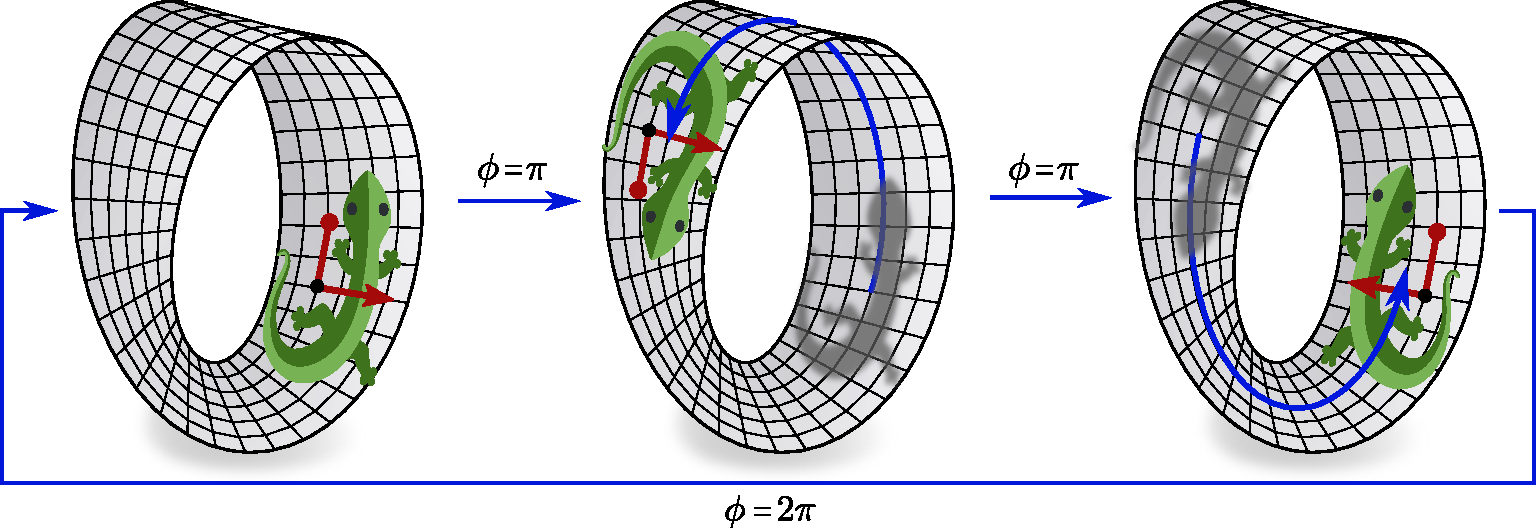
\includegraphics[width=\columnwidth]{figures/mobius_conv_isom.pdf}
	\caption{\small
		تصویری از گروه ایزومتری‌های حافظ ساختار $\Flip$ $\IsomRM$ از نوار موبیوس، که با~$\SO2$ ایزومورف است.
		این گروه شامل تمام دوران‌ها در امتداد نوار است.
		به دلیل پیچش، یک دوران به اندازه $2\pi$ یعنی یک بار به دور نوار، هنوز آن را به خودش باز نمی‌گرداند بلکه منجر به یک بازتاب می‌شود.
		پس از یک دور دوم، یعنی یک دوران کلی $4\pi$، نوار به خودش باز می‌گردد.
		تبدیلات گیج القا شده مقادیری در $\Flip$ می‌گیرند.
		{
			\\ \color{gray} \scriptsize
			(مارمولک‌ها با مجوز \href{https://github.com/twitter/twemoji/blob/gh-pages/LICENSE-GRAPHICS}{\lr{\underline{Creative Commons Attribution 4.0 International}}} با تشکر از توییتر اقتباس شده‌اند.)
		}
	}
	\label{fig:mobius_conv_isometries}
\end{figure}

\subsection{میدان‌های ویژگی مستقل از جهت‌گیری}
\label{sec:mobius_representations}

اصل کوواریانس ایجاب می‌کند که میدان‌های ویژگی روی نوار موبیوس $\RM$-مستقل از مختصات باشند، یعنی باید به طور معادل نسبت به چارچوب‌های هر یک از دو دست‌سانی قابل بیان باشند.
بنابراین آنها با انتخابی از یک نمایش گروهی $\rho: \Flip \to \GL{c}$ از گروه بازتاب مشخص می‌شوند، که تبدیل بردارهای ویژگی عددی را هنگام جابجایی بین دو جهت‌گیری مشخص می‌کند.
ما در ادامه چند انتخاب ممکن از چنین انواع میدانی را مورد بحث قرار خواهیم داد.
خواننده ممکن است بخواهد بررسی کند که نمایش‌های پیشنهادی در واقع همومورفیسم‌های گروهی هستند و در $\rho(gh) = \rho(g)\rho(h),\ \forall g,h\in \Flip$ صدق می‌کنند، همانطور که در بخش~\ref{sec:feature_fields} و پانوشت~\ref{footnote:repr_group_homomorphism} خواسته شده است.

پایه‌ای‌ترین مثال، که برای هر گروه ساختاری وجود دارد، \emph{نمایش بدیهی} است:

\begin{align}
	\rhotriv: \Flip \to \GL{1}\ , \qquad 
	\begin{aligned}
		e &\mapsto \big[\mkern2mu 1 \mkern2mu\big] \\[2pt]
		s &\mapsto \big[\mkern2mu 1 \mkern2mu\big] \\
	\end{aligned}
	\quad ,
\end{align}
که ماتریس همانی {$1\times1$} را به هر دو عنصر گروه اختصاص می‌دهد.
این نمایش، میدان‌های اسکالر $f_{\textup{triv}}$ را مدل می‌کند که شامل بردارهای ویژگی یک‌بعدی هستند که مختصات‌بندی آنها $f^A_{\textup{triv}}(p) \in \R^1$ تحت \emph{بازتاب‌های چارچوب ناوردا} باقی می‌ماند.
دومین نمایش یک‌بعدی، \emph{نمایش علامت-معکوس} است:

\begin{align}
	\rhosign: \Flip \to \GL{1}\ , \qquad 
	\begin{aligned}
		e &\mapsto \big[\mkern2mu 1 \mkern2mu\big] \\[2pt]
		s &\mapsto \big[\! \shortminus\!1 \big]
	\end{aligned}
	\quad .
\end{align}
این نمایش، ماتریس همانی منفی {$1\times1$} را به بازتاب‌ها اختصاص می‌دهد و بنابراین میدان‌های شبه‌اسکالر را توصیف می‌کند، یعنی میدان‌های ویژگی یک‌بعدی $f_{\textup{sign}}$ که ضرایب عددی آنها $f^A_{\textup{sign}}(p) \in \R^1$ \emph{تحت بازتاب‌ها علامت خود را تغییر می‌دهند}، یعنی، $\rhosign(s)\cdot f^A_{\textup{sign}}(p) = -f^A_{\textup{sign}}(p)$.
از آنجا که نمایش بدیهی و نمایش علامت-معکوس یک‌بعدی هستند، هر دو نمایش‌های تحویل‌ناپذیر (irreps) گروه بازتاب هستند.
در واقع، این دو تنها نمایش‌های تحویل‌ناپذیر گروه بازتاب هستند.%
\footnote{
	گروه بازتاب با گروه دوری $\Z/2\Z$ از مرتبه دو ایزومورف است.
	به خوبی شناخته شده است که نمایش‌های تحویل‌ناپذیر گروه‌های دوری از مرتبه $N$ با ریشه‌های $N$-ام واحد مطابقت دارند، که برای $N=2$ فقط $+1$ (بدیهی) و $-1$ (علامت-معکوس) هستند.
}

از آنجا که $\Flip$ یک گروه متناهی است، دارای یک \emph{نمایش منظم} متناهی-بعدی (دو-بعدی) است:

\begin{align}
	\rhoreg: \Flip \to \GL{2}\ , \qquad 
	\begin{aligned}
		e &\mapsto
		\begin{bmatrix} \hspace{1.5pt}
			1 &\mkern-4mu 0 \hspace*{1.5pt} \\ \hspace{1.5pt} 0 &\mkern-4mu 1 \hspace*{1.5pt}
		\end{bmatrix} \\[2pt]
		s &\mapsto 
		\begin{bmatrix} \hspace{1.5pt}
			0 &\mkern-4mu 1 \hspace*{1.5pt} \\ \hspace{1.5pt} 1 &\mkern-4mu 0 \hspace*{1.5pt}
		\end{bmatrix}
	\end{aligned}
	\quad ,
\end{align}
که عناصر گروه را با ماتریس‌های جایگشت نمایش می‌دهد.
بنا به تعریف، نمایش منظم جایگشت عناصر گروه در $\Flip$ را هنگام عمل بر روی خودشان مدل می‌کند.
این را با ستون‌های جدول ضرب در معادله~\eqref{eq:reflection_multiplication_table} مقایسه کنید:
ستون میانی را می‌توان ناشی از عمل $\rhoreg(e)$ بر روی ستون سمت چپ در نظر گرفت، در حالی که عناصر جابجا شده گروه در ستون راست با جایگشت توصیف شده توسط عمل $\rhoreg(s)$ بر روی ستون چپ مطابقت دارد.
میدان‌های ویژگی منظم $f_{\textup{reg}}$ از $\Flip$ به صورت عددی با بردارهای ویژگی دو-بعدی $f^A_{\textup{reg}}(p) \in \R^2$ نمایش داده می‌شوند که دو \emph{کانال آنها تحت بازتاب‌ها جابجا می‌شوند}، یعنی:
$
\rhoreg(s) \mkern-1mu\cdot\mkern-2mu f^A_{\textup{reg}}(p)
\,=\,
\begin{bmatrix} \hspace{1.5pt} 0 &\mkern-4mu 1 \hspace*{1.5pt} \\ \hspace{1.5pt} 1 &\mkern-4mu 0 \hspace*{1.5pt} \end{bmatrix}
\mkern-4mu \cdot\mkern-4mu 
\begin{bmatrix} f^A_{\textup{reg},1} \\ f^A_{\textup{reg},2} \end{bmatrix} \!(p)
\,=\,
\begin{bmatrix} f^A_{\textup{reg},2} \\ f^A_{\textup{reg},1} \end{bmatrix} \!(p)
$.


نمایش منظم تحویل‌پذیر است، یعنی شامل دو زیرفضای ناوردای سره است که در این مورد با نمایش بدیهی و علامت-معکوس مطابقت دارند.
بنابراین می‌توان آن را به طور معادل به صورت ساخته شده از جمع مستقیم $\rhotriv \oplus \rhosign$ از آن دو نمایش تحویل‌ناپذیر و یک تغییر پایه $Q$ در نظر گرفت:

\begin{align}\label{eq:rho_reg_decomposition}
	\rhoreg(g)\ =\ Q\, \big( \rhotriv \!\oplus\mkern-1mu \rhosign \big)\mkern-2mu(g)\; Q^\top
	\quad\ \textup{where } \quad
	Q = \frac{1}{\sqrt{2}}
	\begin{bmatrix} \hspace{1.5pt}
		1 &\mkern-7mu \shortminus1 \hspace*{1.5pt} \\ \hspace{1.5pt} 1 &\mkern-7mu \phantom{\shortminus}1 \hspace*{1.5pt}
	\end{bmatrix}
\end{align}
اعتبار این گزاره به راحتی با قرار دادن سمت راست برای هر دو عنصر گروه تأیید می‌شود:

\begin{align}
	Q\, \big( \rhotriv \!\oplus\mkern-1mu \rhosign \big)\mkern-2mu(e)\; Q^\top
	\ =\ \frac{1}{2}
	\begin{bmatrix} \hspace{1.5pt}
		1 &\mkern-7mu \shortminus1 \hspace*{1.5pt} \\ \hspace{1.5pt} 1 &\mkern-7mu \phantom{\shortminus}1 \hspace*{1.5pt}
	\end{bmatrix} \mkern-6mu \cdot\mkern-6mu
	\begin{bmatrix} \hspace{1.5pt}
		1 &\mkern-7mu 0 \hspace*{1.5pt} \\ \hspace{1.5pt} 0 &\mkern-7mu 1 \hspace*{1.5pt}
	\end{bmatrix} \mkern-6mu \cdot\mkern-6mu
	\begin{bmatrix} \hspace{1.5pt}
		\phantom{\shortminus}1 &\mkern-7mu 1 \hspace*{1.5pt} \\ \hspace{1.5pt} \shortminus1 &\mkern-7mu 1 \hspace*{1.5pt}
	\end{bmatrix}
	\ =\ 
	\begin{bmatrix} \hspace{1.5pt}
		1 &\mkern-7mu 0 \hspace*{1.5pt} \\ \hspace{1.5pt} 0 &\mkern-7mu 1 \hspace*{1.5pt}
	\end{bmatrix}
	\ =\ \rhoreg(e)
\end{align}

\begin{align}
	Q\, \big( \rhotriv \!\oplus\mkern-1mu \rhosign \big)\mkern-2mu(s)\; Q^\top
	\,=\, \frac{1}{2}
	\begin{bmatrix} \hspace{1.5pt}
		1 &\mkern-7mu \shortminus1 \hspace*{1.5pt} \\ \hspace{1.5pt} 1 &\mkern-7mu \phantom{\shortminus}1 \hspace*{1.5pt}
	\end{bmatrix} \mkern-6mu \cdot\mkern-6mu
	\begin{bmatrix} \hspace{1.5pt}
		1 &\mkern-7mu \phantom{\shortminus}0 \hspace*{1.5pt} \\ \hspace{1.5pt} 0 &\mkern-7mu \shortminus1 \hspace*{1.5pt}
	\end{bmatrix} \mkern-6mu \cdot\mkern-6mu
	\begin{bmatrix} \hspace{1.5pt}
		\phantom{\shortminus}1 &\mkern-7mu 1 \hspace*{1.5pt} \\ \hspace{1.5pt} \shortminus1 &\mkern-7mu 1 \hspace*{1.5pt}
	\end{bmatrix}
	\,=\, \frac{1}{2}
	\begin{bmatrix} \hspace{1.5pt}
		1 &\mkern-7mu \phantom{\shortminus}1 \hspace*{1.5pt} \\ \hspace{1.5pt} 1 &\mkern-7mu \shortminus1 \hspace*{1.5pt}
	\end{bmatrix} \mkern-6mu \cdot\mkern-6mu
	\begin{bmatrix} \hspace{1.5pt}
		\phantom{\shortminus}1 &\mkern-7mu 1 \hspace*{1.5pt} \\ \hspace{1.5pt} \shortminus1 &\mkern-7mu 1 \hspace*{1.5pt}
	\end{bmatrix}
	\,=\, 
	\begin{bmatrix} \hspace{1.5pt}
		0 &\mkern-7mu 1 \hspace*{1.5pt} \\ \hspace{1.5pt} 1 &\mkern-7mu 0 \hspace*{1.5pt}
	\end{bmatrix}
	\,=\, \rhoreg(s)
\end{align}
به طور کلی‌تر، هر نمایش متناهی-بعدی از گروه‌های فشرده (شامل گروه‌های متناهی) به طور \emph{کامل قابل تحویل} به یک جمع مستقیم از نمایش‌های تحویل‌ناپذیر است~\cite{gallier2019harmonicRepr,din2017reprLectureNotes,serre1977linear}.
این نشان می‌دهد که هر بردار ویژگی کوواریانت، که تحت یک گروه ساختار فشرده تبدیل می‌شود، تا یک تغییر پایه می‌تواند از ویژگی‌های نمایش تحویل‌ناپذیر ساخته شود.
همانطور که در~\cite{Weiler2019_E2CNN} استدلال شده است، در این مورد در واقع امکان کاهش هر عملیات شبکه \emph{خطی} به عملیات معادل بین میدان‌های نمایش تحویل‌ناپذیر وجود دارد، که ساخت فضای کرنل‌های $G$-راهبر را در معادله~\eqref{eq:G-steerable_kernel_space} و بایاس‌های ناوردا را در معادله~\eqref{eq:gauge_bias_solution_space} ساده می‌کند.
با این حال، همانطور که در ادامه خواهیم دید، انتخاب خاص پایه از انواع میدان معادل، تأثیر کاملاً قابل توجهی بر عملکرد مدل دارد.
دلیل این امر این است که عملیات شبکه \emph{غیرخطی} به پایه انتخاب شده حساس هستند، یعنی به یک انتخاب خاص از انواع میدان معادل.